\chapter{Gestión del proyecto}
\label{anx:gestion}

%%% Revisar las fechas y las horas

La realización de este proyecto comenzó a finales de septiembre de 2011 y se ha prolongado hasta agosto de 2012. A lo largo del mismo se han atravesado las fases de documentación, desarrollo, pruebas y redacción de la memoria. A continuación se muestra una tabla con las distintas fases y el coste en horas de cada una de ellas:

\begin{table}[!htbp]
\centering
   \begin{tabular}{|c|c|c|c|}
      \hline
      \textbf{Fase} & \textbf{Fecha de inicio} & \textbf{Fecha de finalización} & \textbf{Número de horas} \\ \hline
      Documentación & 29/09/2011 & 08/12/2011 & 148 \\ \hline
      Desarrollo & 13/12/2011 & XX/08/2012 & 380 \\ \hline
      Pruebas & 02/05/2012 & 02/07/2012 & 32 \\ \hline
      Memoria & 06/03/2012 & XX/08/2012 & 64 \\ \hline
      \hline
      Número total de horas & 29/09/2011 & XX/08/2012 & XX \\ \hline
   \end{tabular}
\caption{Número de horas invertidas.}
\label{table:horas}
\end{table}

Para ver el desarrollo del proyecto a lo largo de los meses se incluye a continuación un diagrama de Gantt:

\begin{figure} [!htbp]
  \centering
  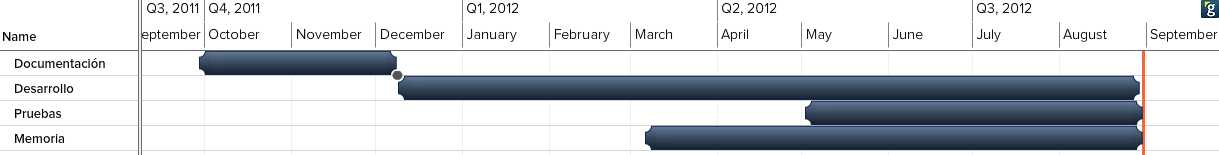
\includegraphics[width=13.5cm]{imagenes/gantt.png}
  \caption{Diagrama de Gantt.}
\label{figure:gantt}
\end{figure}

[Revisar] Hablar de los problemas de AppScale (documentación y bug) y TORQUE (bug del scheduler)
